% -- Slide ---------------------------------------------------------------------
\begin{frame}
\frametitle{\bf Time Profiler}

    \begin{itemize}
        \item Sampling profiler at the level of machine code instructions
        \begin{itemize}
            \item Currently supports fixed and variable-length intervals
            \item Profiling results are currently displayed with the assembly listing
            \item Support for more advanced profiling reports is planned (e.g. HTML report, SeeSoft-like tool, etc.)
        \end{itemize}
    \end{itemize}

    % TODO: screenshot
\end{frame}
% ------------------------------------------------------------------------------

% -- Slide ---------------------------------------------------------------------
\begin{frame}[fragile]
\frametitle{\bf Allocation Profiler}

\begin{itemize}
    \item Allocation profiler currently implemented for the host environment
    \begin{itemize}
        \item Needs to be ported to the bootstrapped environment
        \item Implementation almost entirely in JavaScript
        \item Integration into web-based profiler planned
    \end{itemize}
    \begin{block}<+->{Sample output}
    \begin{lstlisting}[language=]
    Types for Assembly (70.6% bytes accounted for):
        Code: 1197 instances, 118112 bytes
        FixedArray: 650 instances, 59880 bytes
        JSFunctionResultCache: 30 instances, 23440 bytes
        ByteArray: 1197 instances, 15192 bytes
        HeapObject: 300 instances, 3600 bytes
        Primitive: 10 instances, 120 bytes
    \end{lstlisting}
    \end{block}
\end{itemize}
\end{frame}
% ------------------------------------------------------------------------------

% -- Slide ---------------------------------------------------------------------
\begin{frame}
\frametitle{\bf Profile Analyzer}

    \begin{itemize}
        \item Interactive, web-based tool
        \item Uses JSON for profiles
        \item Can easily be extended to support new features
    \end{itemize}

    \begin{center}
        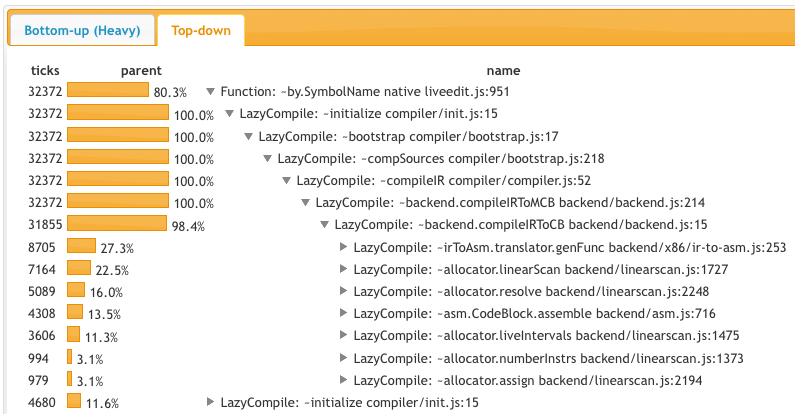
\includegraphics[height=1.5in]{images/prof-topdown.png}
    \end{center}
\end{frame}
% ------------------------------------------------------------------------------

% -- Slide ---------------------------------------------------------------------
\begin{frame}
\frametitle{\bf Debugger}
    \begin{itemize}
        \item Firebug is the current state-of-the-art for debugging JS programs
        \item Can we provide better tools for difficult tasks ?
        \item For example: 
        \begin{itemize}
            \item Heap analysis rather than allocation profiling
            \item Visualisation tools for understanding behaviour
            \item Static analysis tools to verify properties of JS code / find
            errors
            \item Refactoring tools to better support iterative development
        \end{itemize}
    \end{itemize}
\end{frame}
% ------------------------------------------------------------------------------

% -- Slide ---------------------------------------------------------------------
\begin{frame}
\frametitle{\bf Browser Integration}

    \begin{itemize}
        \item Browser integration is necessary to execute real-world JS programs
        \begin{itemize}
            \item Currently investigating possible avenues for Tachyon in a
        production-quality browser
            \item Looked at Safari, Chrome and Firefox APIs
        \end{itemize}
        \item Research questions
        \begin{itemize}
            \item Can we expose Tachyon objects as DOM objects in the browser ?
            \item Could it reduce the DOM barrier cost using a pure JS
            implementation from the browser to the VM ?
        \end{itemize}
    \end{itemize}
\end{frame}
% ------------------------------------------------------------------------------

